\documentclass[12pt]{article}

% MLA format
\usepackage[letterpaper]{geometry}
\usepackage{times}
\geometry{top=1.0in, bottom=1.0in, left=1.0in, right=1.0in}
\usepackage{fancyhdr}
\pagestyle{fancy}
\lhead{} 
\chead{} 
\rhead{Simmons \thepage} 
\lfoot{} 
\cfoot{} 
\rfoot{}
\renewcommand{\headrulewidth}{0pt} 
\renewcommand{\footrulewidth}{0pt} 

\usepackage{mdwlist}
\usepackage{enumitem}
\setlist{  
  listparindent=\parindent,
  parsep=0pt,
}
\title{Homework 5A}
\author{Mark Simmons}
\date{March 6, 2020}

% Multi-line glosses
%\usepackage{chngcntr}
%\usepackage{gb4e,cgloss4e}

%\newcounter{glossnum}

%\newcommand{\numgloss}{\refstepcounter{glossnum}\alph{glossnum}.\space}
%\counterwithin{glossnum}{xnumi}
%\renewcommand{\theglossnum}{\thexnumi\alph{glossnum}}

% Typing in IPA
\usepackage{tipa}

% Sentence trees
\usepackage{tikz-qtree}
\usepackage{lscape}
\usepackage{graphicx}
\tikzset{level distance=30pt,
    sibling distance=6pt,
    every tree node/.style={align=center},
    }

\begin{document}

\maketitle

\begin{enumerate}

% question 1
\item Technical Problem\\

\noindent\resizebox{\textwidth}{!}{\begin{tikzpicture}
{\small \Tree
[.CP {}
[.C' C\\$\emptyset$
[.TP$_{1}$
	[.CP {} [.C' C\\For
		[.TP$_{2}$
		[.NP {} 
		[.N' N\\Bill$_{i}$ {} ] ]%N', NP
		[.T' T\\to [.VP {} [.V' V\\disavow
		[.NP D\\the [.N'
			[.N' N\\photograph$_{j}$
			[.PP {} [.P' P\\of [.NP {} [.N' N\\himself$_{i}$ {} ] ]%N', NP
			] ] ]%P', PP, N'
			[.PP {} [.P' P\\from [.NP {} [.N' N\\yesterday$_{k}$ {}
			] ]%NP, N'
			] ]%P', PP
		] ]%N'. NP
		] ]%V', VP
		] ] %T', TP
	]%C'
	]%CP
	[.\node(T'){T'}; \edge[roof]; {suggests that...} ]
]%TP
]%C'
]%CP
}
\end{tikzpicture}}

\noindent\resizebox{\textwidth}{!}{\begin{tikzpicture}
{\small \Tree
[.T' T\\$\emptyset_{[+PRES]}$
[.VP {} [.V' V\\suggests
	[.CP {} [.C' C\\that
	[.TP$_{3}$ [.NP [.N' N\\he$_{i}$ {} ] ]%N', NP
	[.T' T\\$\emptyset$
		[.VP {} [.V' V\\is [.\node(VP){VP}; \edge[roof]; {willfully perjuring...} ] ] ]%V', VP
	] ]%T', TP
	] ]%C', CP
] ]%V', VP
]%T'
}
\end{tikzpicture}}

\noindent\resizebox{\textwidth}{!}{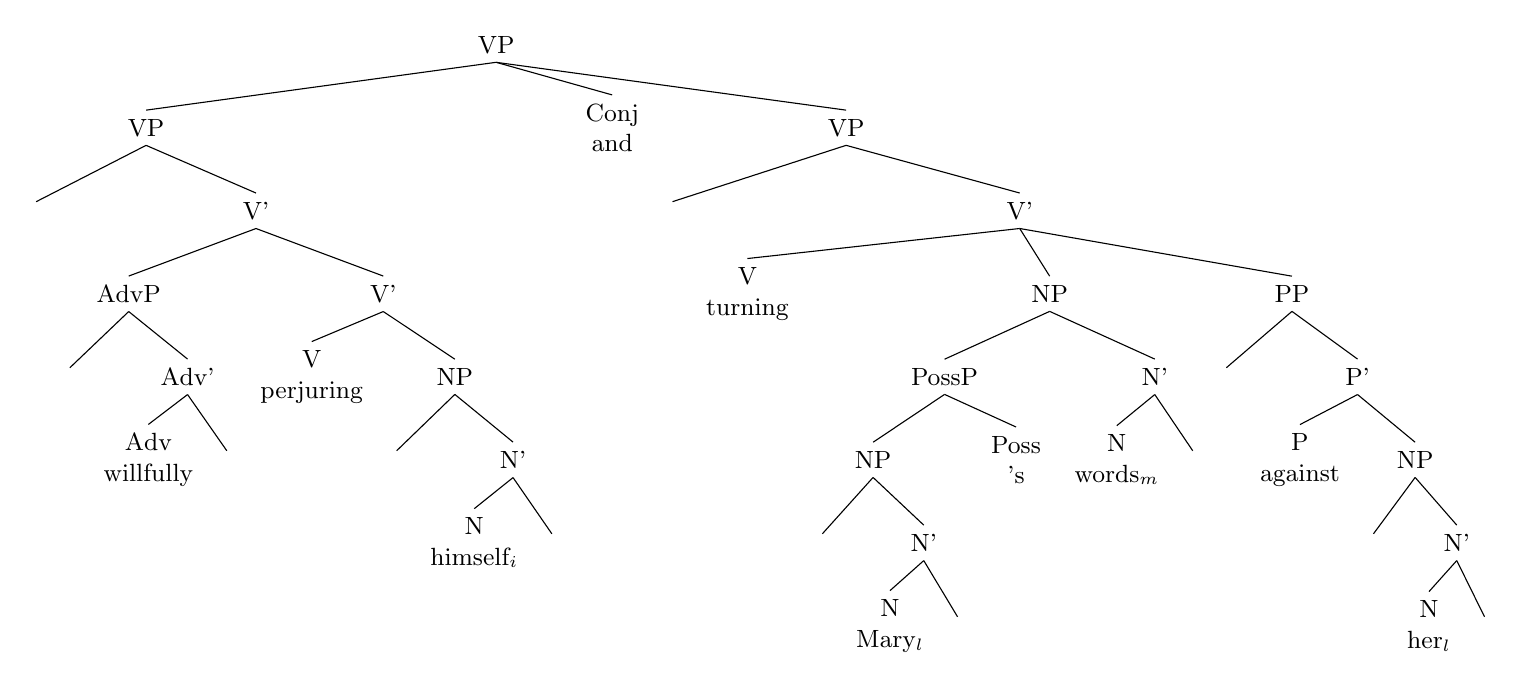
\begin{tikzpicture}
{\small \Tree
[.VP
	[.VP {}
	[.V'
	[.AdvP {} [.Adv' Adv\\willfully {} ] ]%Adv', AdvP
		[.V' V\\perjuring
		[.NP {} [.N' N\\himself$_{i}$ {} ] ]%N', NP
		]%V'
	]%V'
	]%VP
	Conj\\and
	[.VP {}
	[.V' V\\turning
		[.NP [.PossP
			[.NP {} [.N' N\\Mary$_{l}$ {} ] ]%N', NP
		Poss\\'s ]%PossP
		[.N' N\\words$_{m}$ {} 
		] ]%N', NP
		[.PP {} [.P'
		P\\against [.NP {} [.N' N\\her$_{l}$ {} ] ]%N', NP
		] ]%P', PP
	]%V'
	]%VP
]%VP
}
\end{tikzpicture}}

\underline{Binding}
\begin{itemize}
\item \emph{Bill} is an R-expression, thus binding principle C requires that it not be bound. No NP's C-command \emph{Bill}, therefore the binding principle is satisfied.
\item \emph{photograph} is an R-expression, thus binding principle C requires that it not be bound. \emph{Bill} c-commands \emph{photograph}, therefore \emph{Bill} and \emph{photograph} cannot be co-indexed.
\item \emph{himself} is an anaphor, thus binding principle A requires that it be bound within its binding domain. It's binding domain is TP$_{2}$. \emph{Bill} is the only NP that C-commands \emph{himself}, thus \emph{Bill} coindexes 
\emph{himself}, satisfying the binding principle.
\item \emph{yesterday} is an R-expression, thus binding principle C requires that it not be bound. Only \emph{Bill} C-commands \emph{yesterday}, and so the two NPs cannot be coindexed in order for the binding principle to be satisfied.
\item \emph{he} is a pronoun, thus binding principle B requires that it be free within its binding domain. It's binding domain is TP$_{3}$. No NP's under TP$_{3}$ C-command \emph{he}, thus it is free within its binding domain and principle B is satisfied. \emph{he} is coindexed with \emph{Bill}, which is outside the binding domain, being above T$_{3}$.
\item \emph{himself} is an anaphor, thus binding principle A requires that it be bound within its binding domain. It's binding domain is TP$_{3}$. The NP \emph{he} C-commands \emph{himself} in this domain, satisfying the binding principle. Since \emph{he} is coindexed with \emph{Bill} outside the binding domain, \emph{himself} is coindexed with \emph{Bill} and \emph{he}.
\item \emph{Mary} is an R-expression, thus binding principle C requires that it not be bound. The only NP that C-commands \emph{Mary} is the pronoun \emph{he}, therefore these NPs cannot be coindexed, leaving \emph{Mary} free.
\item \emph{her} is a pronoun, thus binding principle B requires that it be free within its binding domain. It's binding domain is TP$_{3}$. The only NP that C-commands \emph{Mary} is the pronoun \emph{he}, therefore these NPs cannot be coindexed, leaving \emph{her} free within its binding domain. \emph{her} is coindexed by \emph{Mary}. Since \emph{Mary} is dominated by the NP \emph{Mary's words}, which does not dominate \emph{her}, \emph{Mary} does not bind \emph{her} and binding principle B is satisfied.
\end{itemize}
\item Argumentation\\

English has a set of ditransitive verbs where both direct and indirect object NPs are expressed immediately following the verb with no preposition or other morphology distinguishing them. Our current grammar model classifies these two objects as complements of the V argument, as seen in trees (1a,b).\\

\pagebreak
\begin{itemize}
\item[(1)]
\begin{enumerate}[label=\alph*.]
\item \leavevmode\vadjust{\vspace{-\baselineskip}}\newline
\noindent{\begin{tikzpicture}
{\small \Tree
[.CP {}
[.C' {}
[.TP [.NP {} [.N' N\\Harrison {} ] ]%N' NP 
[.T' T\\\emph{-ed}
[.VP {} [.V' V\\show
	[.NP D\\the [.N' N\\android$_{i}$ {} ] ]%N', NP
	[.NP D\\a [.N' N\\duplicate [.PP {} [.P' P\\of [.NP {} [.N' N\\itself$_{i}$. {} ] ] ] ] ] ]%N', NP, P', PP, N', NP
] ]%V', VP
]%T'
]%TP
]%C'
]%CP
}
\end{tikzpicture}}\\
\pagebreak
\item \leavevmode\vadjust{\vspace{-\baselineskip}}\newline
\noindent{\begin{tikzpicture}
{\small \Tree
[.CP {}
[.C' {}
[.TP [.NP {} [.N' N\\Harrison {} ] ]%N' NP 
[.T' T\\\emph{-ed}
[.VP {} [.V' V\\show
	[.NP {} [.N' N\\her$_{i}$ {} ] ]%N', NP
	[.NP {} [.N' N\\herself$_{i}$. {} ] ]%N', NP
] ]%V', VP
]%T'
]%TP
]%C'
]%CP
}
\end{tikzpicture}}

\end{enumerate}
\suspend{itemize}

I will argue based on English data of coindexing between these two complements that the tree structure in (1a,b) should be revised. The arguments presented will refer to binding between these two NPs specifically. The binding domain for these NPs is the immediately dominating TP. Since this is the only TP considered in the argument, no further references to binding domain will be made. Similarly, no references will be made to any form of coindexing except for that between the anaphor and the other NP objects of the verb \emph{show} in either sentence.

Since the two objects C-command each other, the direct object (\emph{the android} in (1a), \emph{her} in (1b)) can legally bind the anaphor (\emph{itself} in (1a), \emph{herself} in (1b)), satisfying Binding Principle A which requires the anaphor to be bound within its domain. This enables our grammar to produce the correctly-indexed sentences (1a,b) - however, our model also overgenerates since it predicts that the binding can go in the opposite direction, as demonstrated below.

\pagebreak
\resume{itemize}
\item[(2)]
\begin{enumerate}[label=\alph*.]
\item \leavevmode\vadjust{\vspace{-\baselineskip}}\newline
\noindent{\begin{tikzpicture}
{\small \Tree
[.CP {}
[.C' {}
[.TP [.NP {} [.N' N\\Harrison {} ] ]%N' NP 
[.T' T\\\emph{-ed}
[.VP {} [.V' V\\show
	[.NP {} [.N' N\\*herself$_{i}$ {} ] ]%N', NP
	[.NP {} [.N' N\\her$_{i}$. {} ] ]%N', NP
] ]%V', VP
]%T'
]%TP
]%C'
]%CP
}
\end{tikzpicture}}

\end{enumerate}
\suspend{itemize}

Sentence (2a) is ungrammatical, but nevertheless our model predicts it as acceptable. This is because the C-command relationship is symmetrical - either object can bind the other. Nothing in the syntactic structure is able to prevent the second object from binding an anaphor that precedes it, even though doing so produces an unacceptable sentence. The same is true of sentence (3a).

\pagebreak
\resume{itemize}
\item[(3)]
\begin{enumerate}[label=\alph*.]
\item \leavevmode\vadjust{\vspace{-\baselineskip}}\newline
\noindent{\begin{tikzpicture}
{\small \Tree
[.CP {}
[.C' {}
[.TP [.NP {} [.N' N\\Harrison {} ] ]%N' NP 
[.T' T\\\emph{-ed}
[.VP {} [.V' V\\show
	[.NP D\\a [.N' N\\duplicate [.PP {} [.P' P\\of [.NP {} [.N' N\\*itself$_{i}$. {} ] ] ] ] ] ]%N', NP, P', PP, N', NP
	[.NP D\\the [.N' N\\android$_{i}$ {} ] ]%N', NP
] ]%V', VP
]%T'
]%TP
]%C'
]%CP
}
\end{tikzpicture}}\\

\end{enumerate}
\suspend{itemize}

Again, because both objects are sisters to V, and thus are sisters to each other, our model incorrectly predicts that the NP \emph{the android} C-commands \emph{itself} even when placed after.

The ungrammaticality of these two sentences suggests that the indirect object, which immediately follows the V, C-commands the direct object, which follows it, but that the direct object does not C-command the preceding indirect object in turn. We can realize this assymetry in the syntax by making the direct object the niece of the indirect object, which can be accomplished by means of a PP with a null head. Since we are only concerned with the syntax of the V and its complements, only the tree for V' will be displayed from here on.

\pagebreak
\resume{itemize}
\item[(4)]
\begin{enumerate}[label=\alph*.]
\item \leavevmode\vadjust{\vspace{-\baselineskip}}\newline
\noindent{\begin{tikzpicture}
{\small \Tree
[.V' V\\show
	[.PP
	[.NP D\\the [.N' N\\android$_{i}$ {} ] ]%N', NP
	[.P' P\\$\emptyset$
	[.NP D\\a [.N' N\\duplicate [.PP {} [.P' P\\of [.NP {} [.N' N\\itself$_{i}$. {} ] ] ] ] ] ]%N', NP, P', PP, N', NP
	]%P'	
	]%PP
]%V'
}
\end{tikzpicture}}\\
\item \leavevmode\vadjust{\vspace{-\baselineskip}}\newline
\noindent{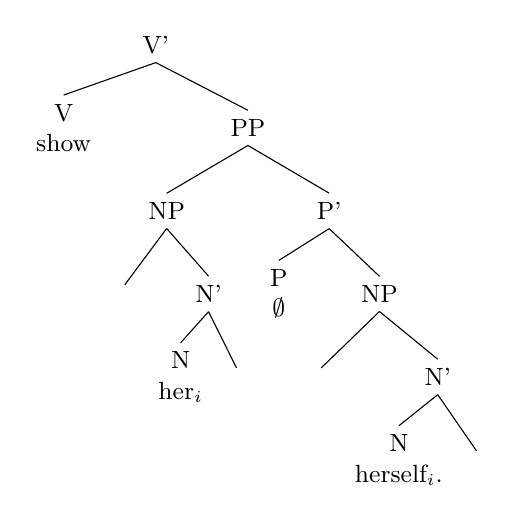
\begin{tikzpicture}
{\small \Tree
[.V' V\\show
	[.PP	
	[.NP {} [.N' N\\her$_{i}$ {} ] ]%N', NP
	[.P' P\\$\emptyset$
	[.NP {} [.N' N\\herself$_{i}$. {} ] ]%N', NP
	]%P'	
	]%PP
]%V'
}
\end{tikzpicture}}

\end{enumerate}
\suspend{itemize}

The indirect object NP is placed in the specifier position of the PP, and the direct object is placed as a complement to the null P argument. Under this model, the C-command is assymetrical; the second object is the niece of the first. Thus when the NPs are reversed, our model accurately predicts that binding is ungrammatical.

\pagebreak
\resume{itemize}
\item[(5)]
\begin{enumerate}[label=\alph*.]
\item \leavevmode\vadjust{\vspace{-\baselineskip}}\newline
\noindent{\begin{tikzpicture}
{\small \Tree
[.V' V\\show
	[.PP
	[.NP D\\a [.N' N\\duplicate [.PP {} [.P' P\\of [.NP {} [.N' N\\*itself$_{i}$. {} ] ] ] ] ] ]%N', NP, P', PP, N', NP
	[.P' P\\$\emptyset$
	[.NP D\\the [.N' N\\android$_{i}$ {} ] ]%N', NP
	]%P'	
	]%PP
]%V'
}
\end{tikzpicture}}\\
\item \leavevmode\vadjust{\vspace{-\baselineskip}}\newline
\noindent{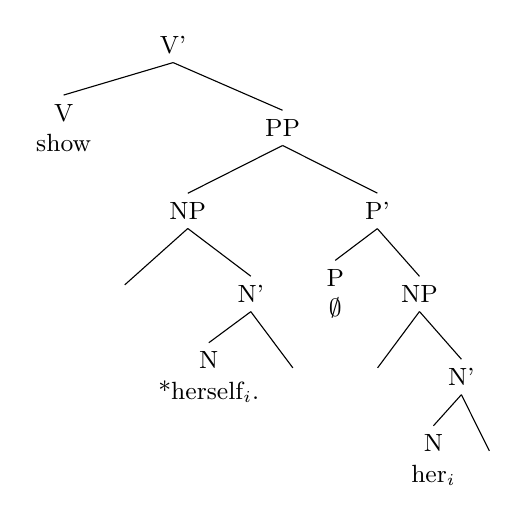
\begin{tikzpicture}
{\small \Tree
[.V' V\\show
	[.PP	
	[.NP {} [.N' N\\*herself$_{i}$. {} ] ]%N', NP
	[.P' P\\$\emptyset$
	[.NP {} [.N' N\\her$_{i}$ {} ] ]%N', NP
	]%P'	
	]%PP
]%V'
}
\end{tikzpicture}}

\end{enumerate}
\suspend{itemize}

In (5a,b), the direct object cannot bind the anaphor \emph{itself} or \emph{herself}. Because the direct object is now dominated by a P' which does not dominate the indirect object (which is sister to P'), the direct object no longer C-commands the indirect object that precedes it. Because of this, our model now matches the actual English distribution of anaphors within ditransitive verb complements more closely.

\item Short Argumentation

This new model is not airtight, however. Since both objects are dominated by a single node, they are predicted to behave as a single constituent. However, as the data in (6a,b) demonstrate, this is not the case.

\resume{itemize}
\item[(6)]
\begin{enumerate}[label=\alph*.]
\item I gave Bill candy.
\item *It was Bill candy I gave.
\item *Bill candy, I gave!
\end{enumerate}
\suspend{itemize}

The grammatical sentence (6a) does not allow the two objects to be clefted, as the unacceptable sentences (6b,c) demonstrate. This contradicts our assumption that the direct and indirect object act as a single constituent dominated by a single PP node complement to the V \emph{gave}.

The sentence likewise does not support both objects being replaced by a single pronoun.

\resume{itemize}
\item[(7)]
\begin{enumerate}[label=\alph*.]
\item I gave Bill candy.
\item *I gave there/so/him/it.
\end{enumerate}
\suspend{itemize}

Nor can both objects be given as a response to a question.

\resume{itemize}
\item[(8)]
\begin{enumerate}[label=\alph*.]
\item *What/who/where did you give?
\item *Bill candy.
\end{enumerate}
\suspend{itemize}

Neither the question itself, where the interrogative pronoun fills the syntactic role of both objects, nor the response, where both objects are given as if a single constituent, form grammatical utterances. Questions that target only one object, however, are grammatical.

\resume{itemize}
\item[(9)]
\begin{enumerate}[label=\alph*.]
\item What did you give Bill?
\item Candy.
\item Who did you give candy?
\item Bill.
\end{enumerate}
\suspend{itemize}

Interestingly, both objects do pass a coordination test.

\resume{itemize}
\item[(9)]
\begin{enumerate}[label=\alph*.]
\item I gave Bill candy.
\item I gave Sandy a flower.
\item I gave Bill candy and Sandy a flower.
\end{enumerate}
\suspend{itemize}

However, as stated in class, coordination can sometimes target multiple constituents at a time and should not be viewed as sufficient evidence of constituency independently.

Therefore, it would seem our solution to the issue of binding relations within ditransitive objects produced an undesired side effect by predicting that the two arguments formed a single constituent.

\item A simple solution to this issue might be to keep the original tree structure (with two sister NP complements), but add an addendum to our definition of binding stating that NPs can only be bound by elements to their left. This is consistent with the fact that English is overwhelmingly a right-branching language, and only in instances such as these do we see arguments C-commanded by arguments to their right.

\item Han Solo did shoot first, so he would probably win. However, let's not forget that bounty hunter Rick Deckard managed to put a laser through the skull of an android that was attempting to "break [his] pencil neck" while in the passenger seat of the car he was driving, so I'd concede this duel to him. Case in point, books are better than movies.

\end{enumerate}
\end{document}
